\documentclass[twoside]{article}
\usepackage[a4paper]{geometry}
\geometry{verbose,tmargin=2.5cm,bmargin=2cm,lmargin=2cm,rmargin=2cm}
\usepackage{fancyhdr}
\pagestyle{fancy}

% nastavení pisma a~češtiny
\usepackage{lmodern}
\usepackage[T1]{fontenc}
\usepackage[utf8]{inputenc}
\usepackage[czech]{babel}

% odkazy
\usepackage{url}

\usepackage{float}
% vícesloupcové tabulky
\usepackage{multirow}
\usepackage{listings}
\usepackage{xcolor}
\usepackage{amssymb}
\usepackage{gensymb}
\usepackage{bbold}
\usepackage{amsmath}
\usepackage{siunitx}
\usepackage{mathtools}
\usepackage{commath}

% vnořené popisky obrázků
\usepackage{subcaption}

% automatická konverze EPS 
\usepackage{graphicx} 
\usepackage{epstopdf}
\epstopdfsetup{update}

\graphicspath{{./images}}

% odkazy a~záložky
\usepackage[unicode=true, bookmarks=true,bookmarksnumbered=true,
bookmarksopen=false, breaklinks=false,pdfborder={0 0 0},
pdfpagemode=UseNone,backref=false,colorlinks=true] {hyperref}


% Poznámky při překladu
\usepackage{xkeyval}	% Inline todonotes
\usepackage[textsize = footnotesize]{todonotes}
\presetkeys{todonotes}{inline}{}

%https://tex.stackexchange.com/questions/2783/bold-calligraphic-typeface
\DeclareMathAlphabet\mathbfcal{OMS}{cmsy}{b}{n}

% enumerate zacina s pismenem
\renewcommand{\theenumi}{\alph{enumi}}

% smaz aktualni page layout
\fancyhf{}
% zahlavi
\usepackage{titling}
\fancyhf[HC]{\thetitle}
\fancyhf[HLE,HRO]{\theauthor}
\fancyhf[HRE,HLO]{\today}
 %zapati
\fancyhf[FLE,FRO]{\thepage}

% údaje o autorovi
\title{OTE Domácí úkol 3b - Přístrojový zesilovač}
\author{Vojtěch Michal}
\date{\today}

%customize code listing
\definecolor{codegreen}{rgb}{0,0.6,0}
\definecolor{codegray}{rgb}{0.5,0.5,0.5}
\definecolor{codepurple}{rgb}{0.58,0,0.82}
\definecolor{backcolour}{rgb}{0.95,0.95,0.92}

\lstdefinestyle{mystyle}{
    backgroundcolor=\color{backcolour},   
    commentstyle=\color{codegreen},
    keywordstyle=\color{magenta},
    numberstyle=\tiny\color{codegray},
    stringstyle=\color{codepurple},
    basicstyle=\ttfamily\footnotesize,
    breakatwhitespace=false,         
    breaklines=true,                 
    captionpos=b,                    
    keepspaces=true,                 
    numbers=left,                    
    numbersep=5pt,                  
    showspaces=false,                
    showstringspaces=false,
    showtabs=false,                  
    tabsize=2
}

\lstset{style=mystyle}

\begin{document}

\maketitle

V simulacích pro tuto úlohu bylo použito nastavení parametrů operačního zesilovače uvedené v tabulce \ref{tab:oz_param}.
Symbolem $u_3$ označuji napětí na výstupu přístrojového zesilovače proti zemi,
napětí $u_2$ a $u_1$ jsou po řadě napětí kladného a záporného vstupu přístrojového zesilovače proti zemi
(konvence použitá v zadání). Struktura symetrického přístrojového zesilovače je na obrázku \ref{fig:instrument_amp}.

\begin{table}[h!]
    \centering
    \begin{tabular}{c|c|c|c|c}
        parametr & symbol & hodnota & jednotka & poznámka\\
        \hline
        Vstupní napěťový offset & $U_0$ & 1 & \si{\milli\volt} & \\
        Vstupní klidový proud & $I_\text{B}$ & 50 & \si{\nano\ampere} & $(I_\text{BP} + I_\text{BN})/2$ \\
        Vstupní zbytkový proud & $I_0$ & 20 & \si{\nano\ampere} & $I_\text{BP} - I_\text{BN}$ \\
        Zesílení v otevřené smyčce & $A_\text{D}$ & 200 & \si{\kilo\volt\per\volt} & \\
        Tranzitní kmitočet& $f_T$ & 1 & \si{\mega\hertz} &
    \end{tabular}
    \caption{Parametry operačního zesilovače použité pro simulaci}
    \label{tab:oz_param}
\end{table}

\begin{figure}[h!]
    \centering
    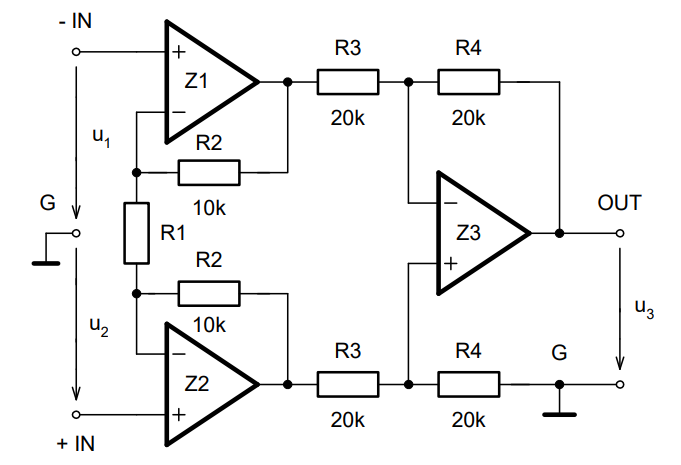
\includegraphics[width=0.8\linewidth]{instrumentation_amp.png}
    \caption{Struktura přístrojového zesilovače, převzato ze zadání}
    \label{fig:instrument_amp}
\end{figure}


\section{Použité rezistory}

Pro rozdílové zesílení přístrojového zesilovače platí vztah
\begin{equation}
    G_\text{D} = \frac{R_4}{R_3}\left(1 2 +\frac{R_2}{R_1}\right).
\end{equation}
Fixováním $R_2 = 10 \si{\kilo\ohm}$ a $R_4 = R_3 = 20 \si{\kilo\ohm}$
je možné plně ovládat rozdílové zesílení nastavováním hodnoty $R_1$.
Potřebné hodnoty odporu $R_1$ pro daná rozdílová zesílení $G_\text{D}$ jsou v tabulce \ref{tab:R}.

\begin{table}
    \centering
    \begin{tabular}{c|c}
        rozdílové zesílení $G_\text{D}$ & $R_1$ [\si{\kilo\ohm}] \\
        \hline
        1 & $\infty$ (rozpojený obvod)\\
        2 & 20\\
        4 & $6,\bar{6}$ \\
        8 & 2,86
    \end{tabular}
    \caption{Hodnoty $R_1$ v závislosti na potřebném rozdílovém zesílení $G_\text{D}$}
    \label{tab:R}
\end{table}

\section{Chyba zesílení a nuly}

Výstupní zbytkové napětí (chyba nuly) změřené při zkratovaných vstupech přístrojového zesilovače je $U_{30} = -2,4 \si{\milli\volt}$
a není závislé na nastavení rozdílového zesílení.

\section{Frekvenční charakteristika rozdílového zesílení $G_\text{D}$}

S pomocí zapojení na schématu \ref{fig:schema_diff_bode} a funkce \textit{AC sweep} byly
získány frekvenční charakteristiky rozdílového zesílení pro $G_\text{D} \in \left\{1, 8\right\}$,
které jsou vykresleny na obrázkách \ref{fig:bode_diff_1} a \ref{fig:bode_diff_8}.
Mezní kmitočty pro jednotlivá zesílení jsou zanesena v tabulce \ref{tab:mezni_f}
a přibližně odpovídají analytickému vztahu pro \textit{gain-bandwidth product} $f_m \cdot (G_\text{D} + 1) = f_T$,
tedy přibližně odpovídají příslušnému rozdílovému zesilovači analyzovanému v minulém domácím úkolu.

Jen pro zesílení $G_\text{D}=1$ je mezní frekvence výrazně nižší než u samotného rozdílového zesilovače,
zejména proto, že rozdílový zesilovač $\text{U}_1$ se zesílením 1 obsažený v přístrojovém zesilovači má na 500 \si{\kilo\hertz}
vlastní mezní frekvenci a pokles zesílení o 3 \si{\deci\bel} proto nastává dříve.

\begin{figure}[h!]
    \centering
    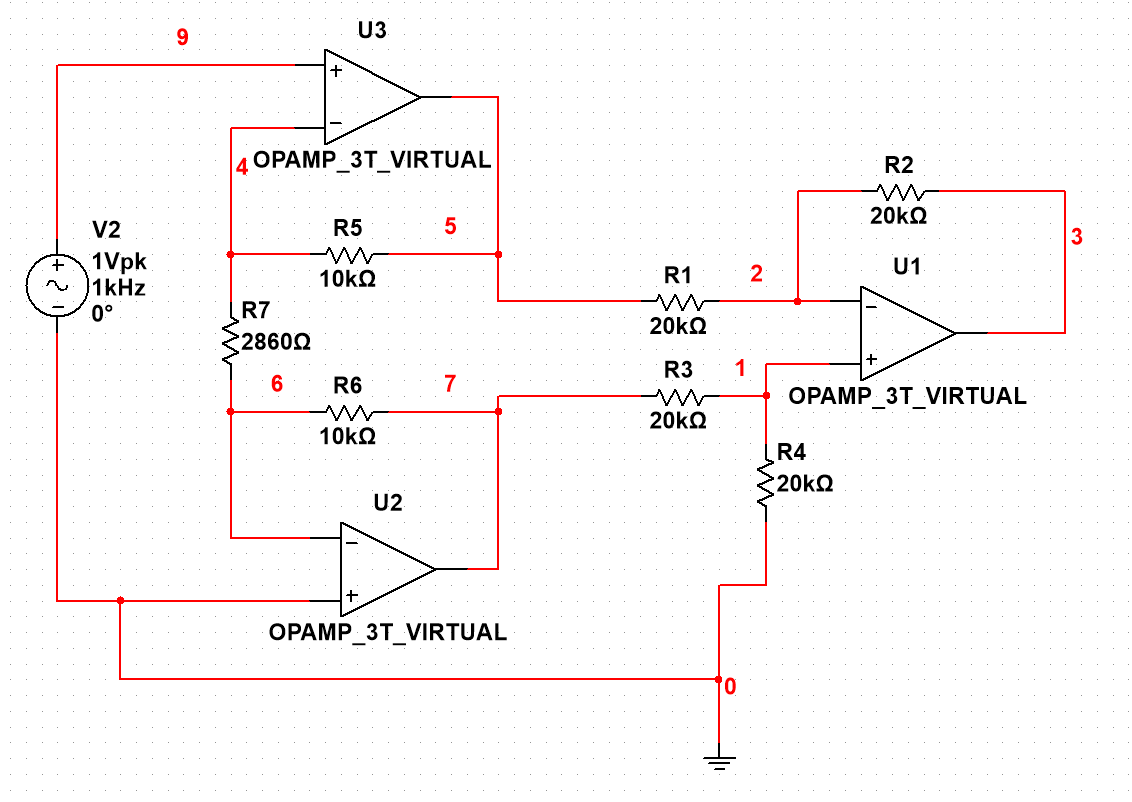
\includegraphics[width=0.8\linewidth]{bode_diff_schema.png}
    \caption{Zapojení pro získání frekvenční charakteristiky rozdílového zesílení $G_\text{D}$}
    \label{fig:schema_diff_bode}
\end{figure}

\begin{table}[h!]
    \centering
    \begin{tabular}{c|c}
        rozdílové zesílení $G_\text{D}$ & mezní kmitočet $f_m$ [\si{\kilo\hertz}] \\
        \hline
        1 & 417 \\
        2 & 324 \\
        4 & 208 \\
        8 & 118 
    \end{tabular}
    \caption{Závislost mezní frekvence na rozdílovém zesílení}
    \label{tab:mezni_f}
\end{table}

\begin{figure}[h!]
    \centering
    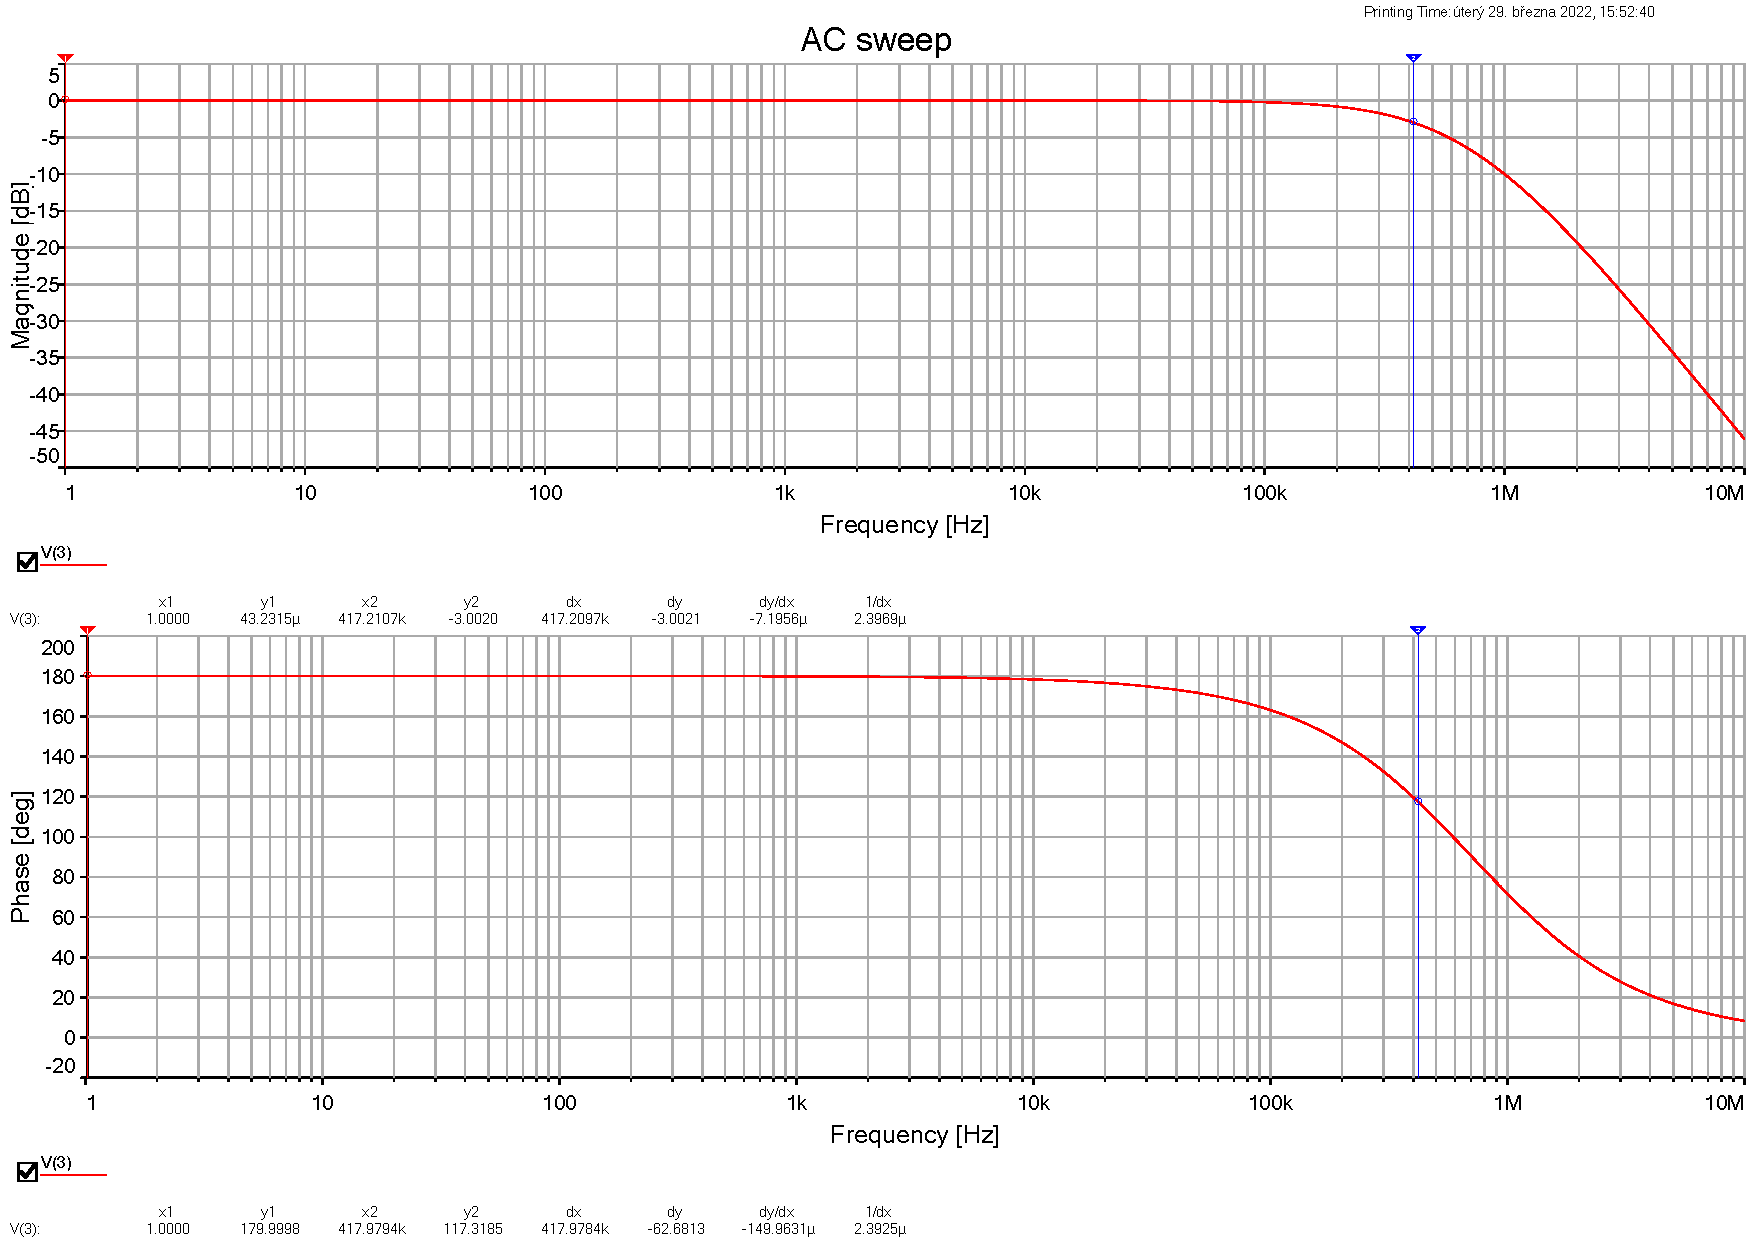
\includegraphics[width=0.92\linewidth]{bode_diff_1.pdf}
    \caption{Frekvenční charakteristika rozdílového zesílení pro $G_\text{D} = 1$}
    \label{fig:bode_diff_1}
\end{figure}

\begin{figure}[h!]
    \centering
    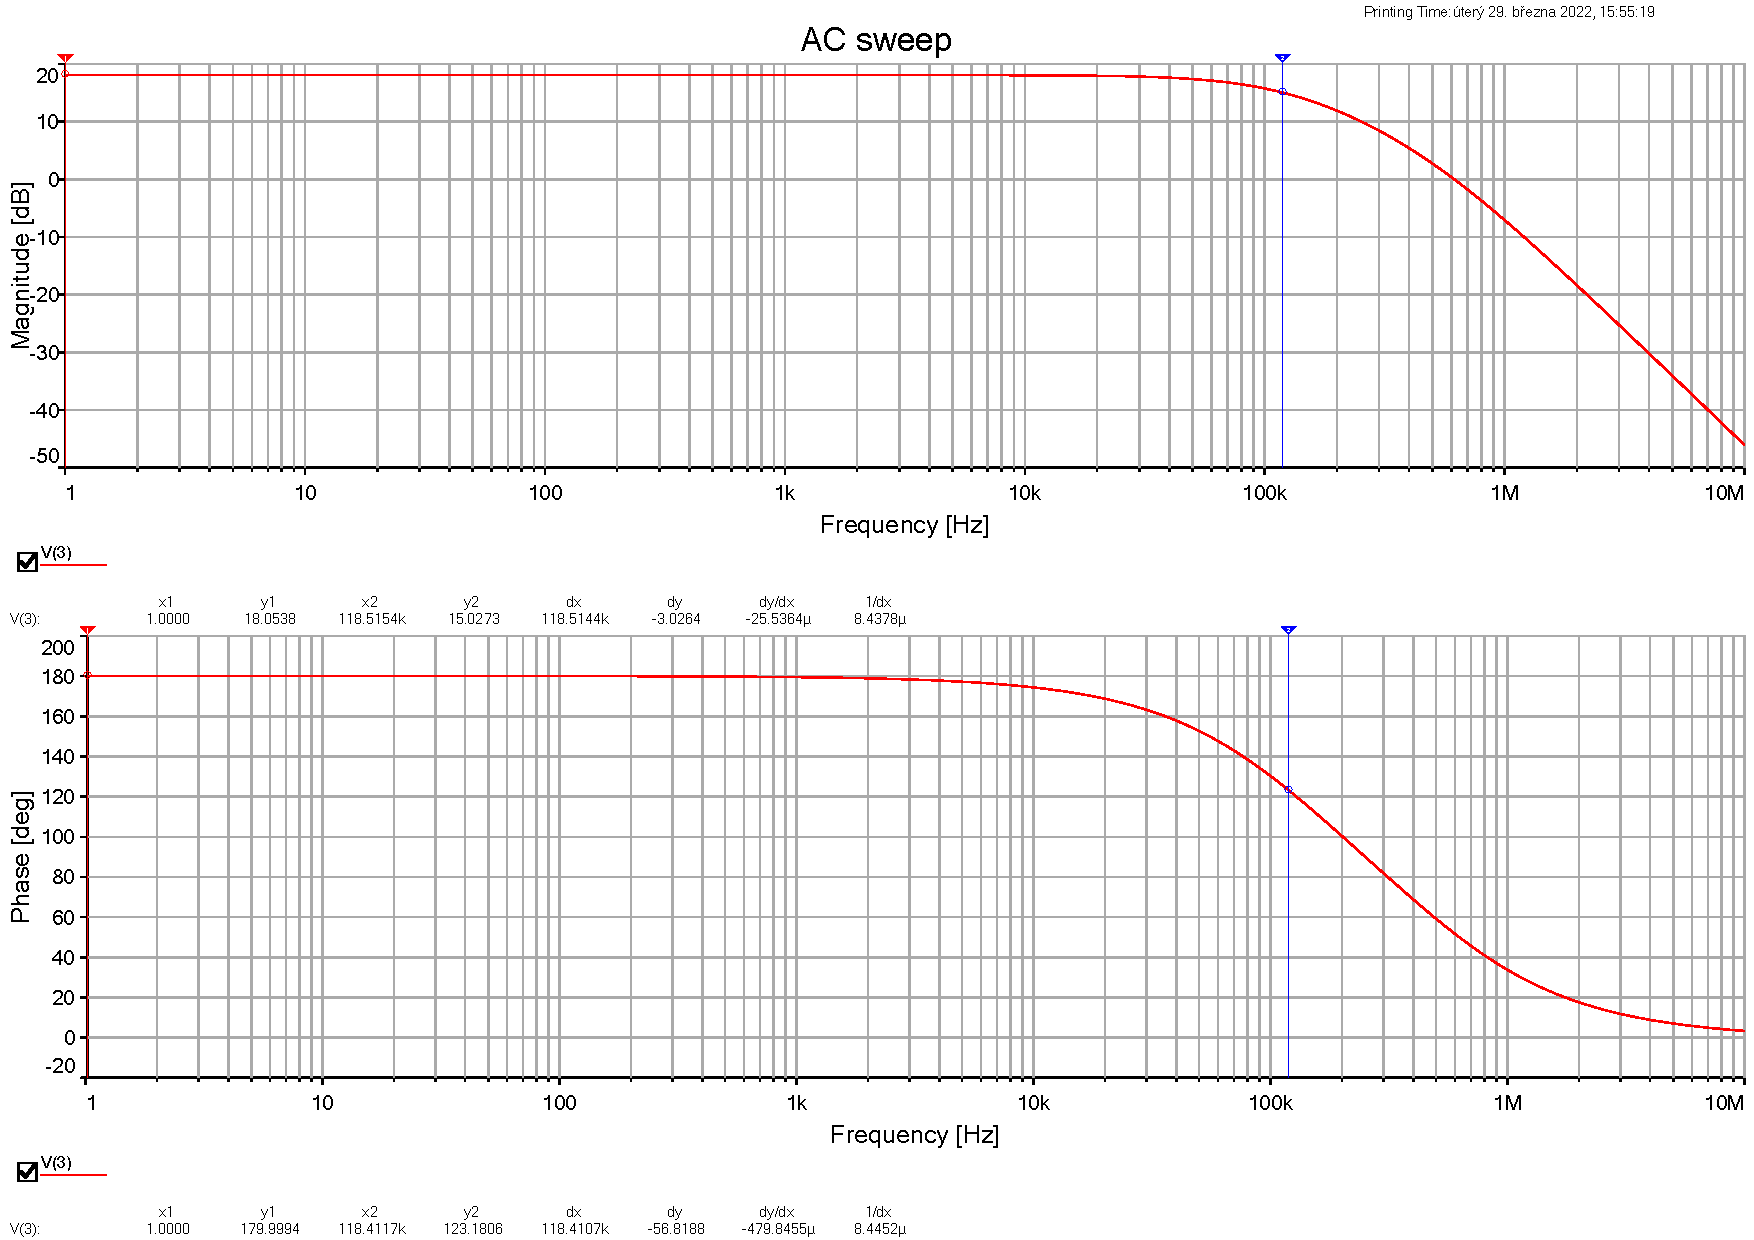
\includegraphics[width=0.92\linewidth]{bode_diff_8.pdf}
    \caption{Frekvenční charakteristika rozdílového zesílení pro $G_\text{D} = 8$}
    \label{fig:bode_diff_8}
\end{figure}

\newpage
\section{Frekvenční charakteristika souhlasného zesílení $G_\text{C}$}

\begin{figure}[h!]
    \centering
    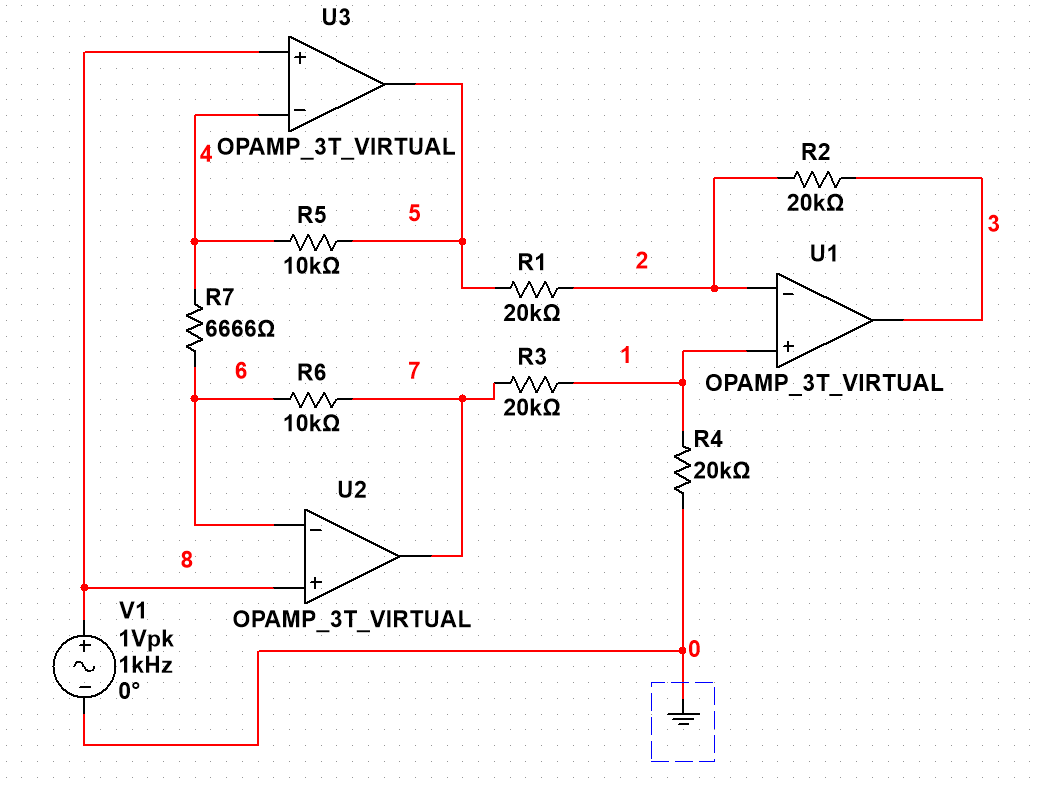
\includegraphics[width=0.8\linewidth]{bode_common_schema.png}
    \caption{Zapojení pro získání frekvenční charakteristiky souhlasného zesílení $G_\text{C}$}
    \label{fig:schema_common}
\end{figure}

S pomocí zapojení na schématu \ref{fig:schema_common} a funkce \textit{AC sweep} byly
získány frekvenční charakteristiky souhlasného zesílení pro $G_\text{D} \in \left\{ 1,8 \right\}$,
které jsou vykresleny na obrázkách \ref{fig:bode_common_1} a \ref{fig:bode_common_8}.

Mezní kmitočet je jen málo závislý na rozdílovém zesílení a pohybuje se kolem 280 \si{\kilo\hertz}, 
tehdy je souhlasné zesílení cca - 78 \si{\deci\bel} bez ohledu na rozdílové zesílení.
Frekvenční charakteristika je podobná pásmové propusti - kmitočty kolem 1 \si{\mega\hertz} jsou propouštěny lépe
než nižší i vyšší. Pro nízké frekvence (DC až 10\si{\hertz}) se souhlasné zesílení pohybuje kolem -160 \si{\deci\bel}.
Proto pro $f\to\infty$ je $\text{CMRR} = 170 \si{\deci\bel}$ i víc, zatímco pro $f \approx 1\si{\mega\hertz}$ je $\text{CMRR} \approx 70 \si{\deci\bel}$.

\begin{figure}[h!]
    \centering
    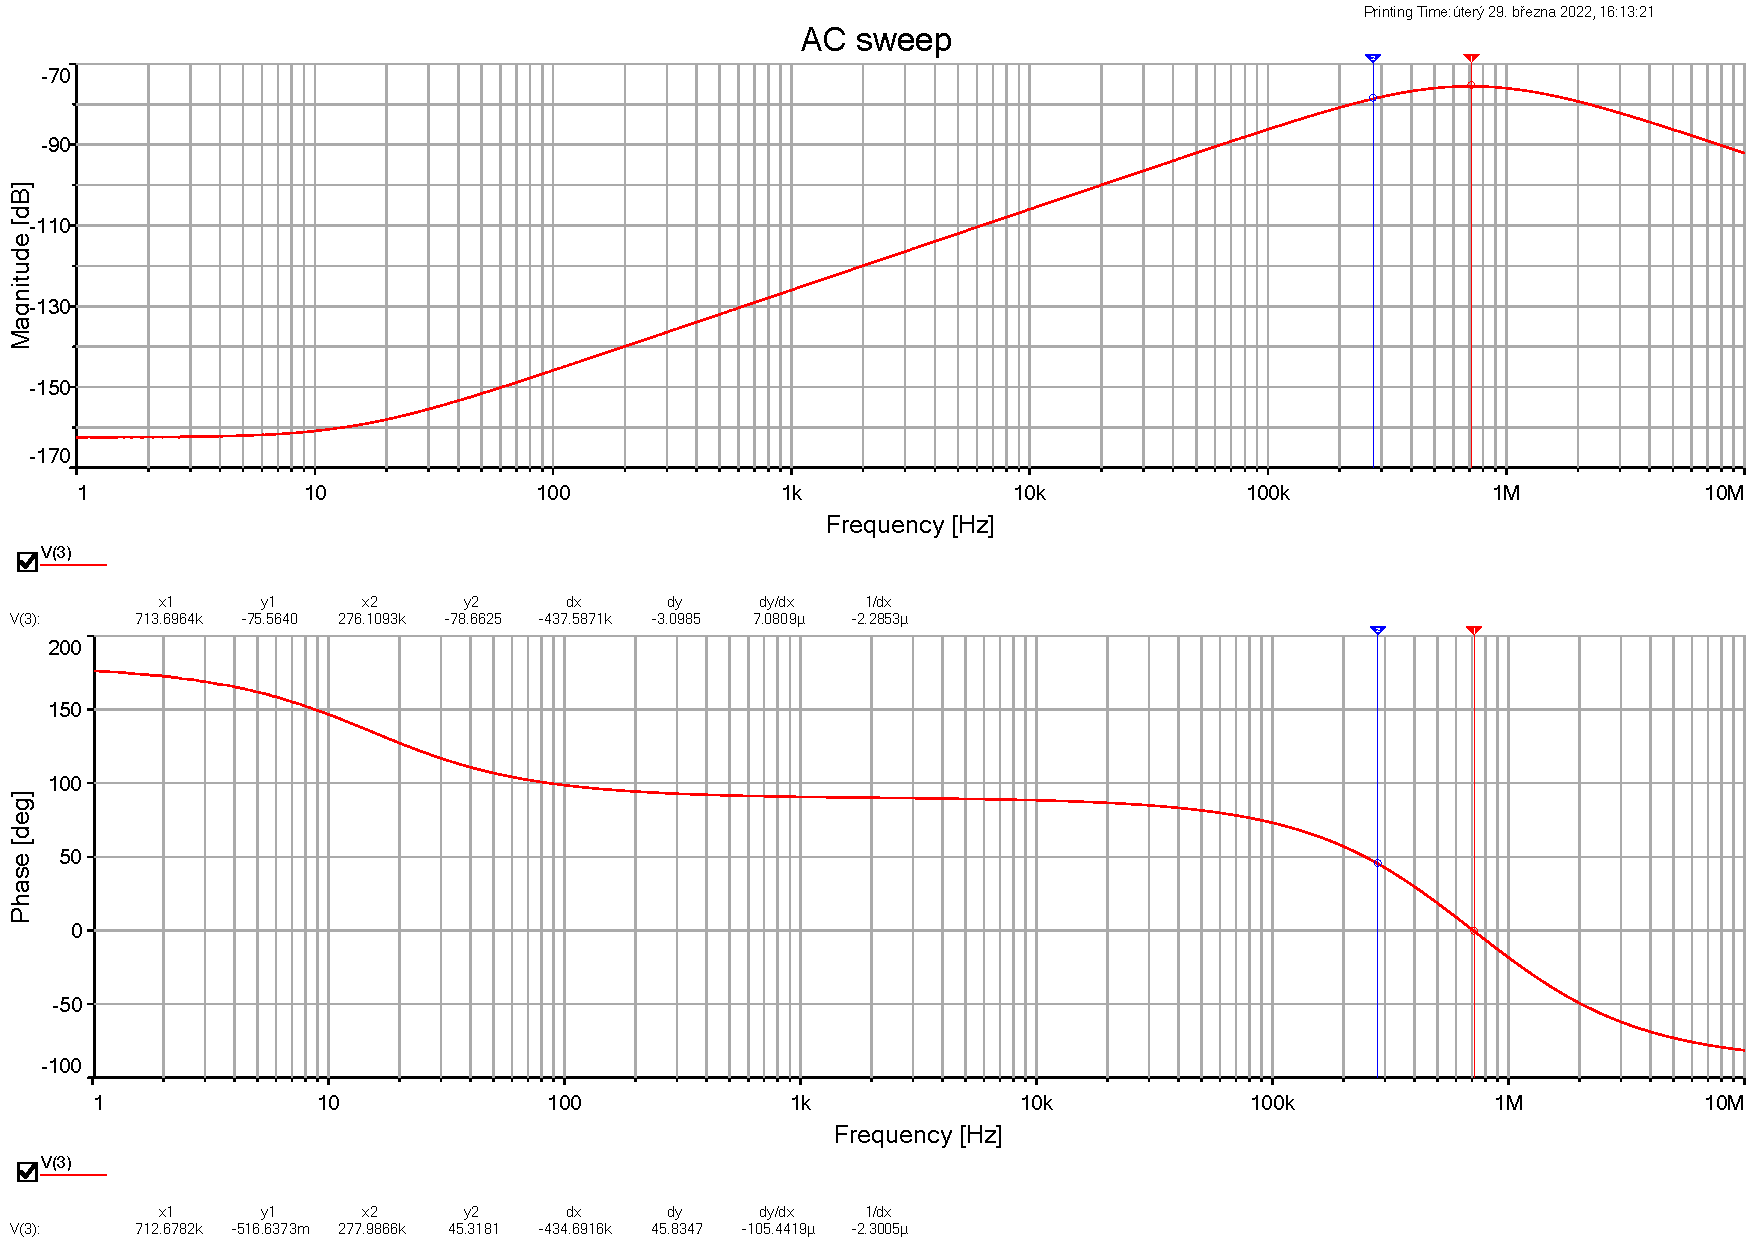
\includegraphics[width=0.92\linewidth]{bode_common_1.pdf}
    \caption{Frekvenční charakteristika souhlasného zesílení pro $G_\text{D} = 1$}
    \label{fig:bode_common_1}
\end{figure}

\begin{figure}[h!]
    \centering
    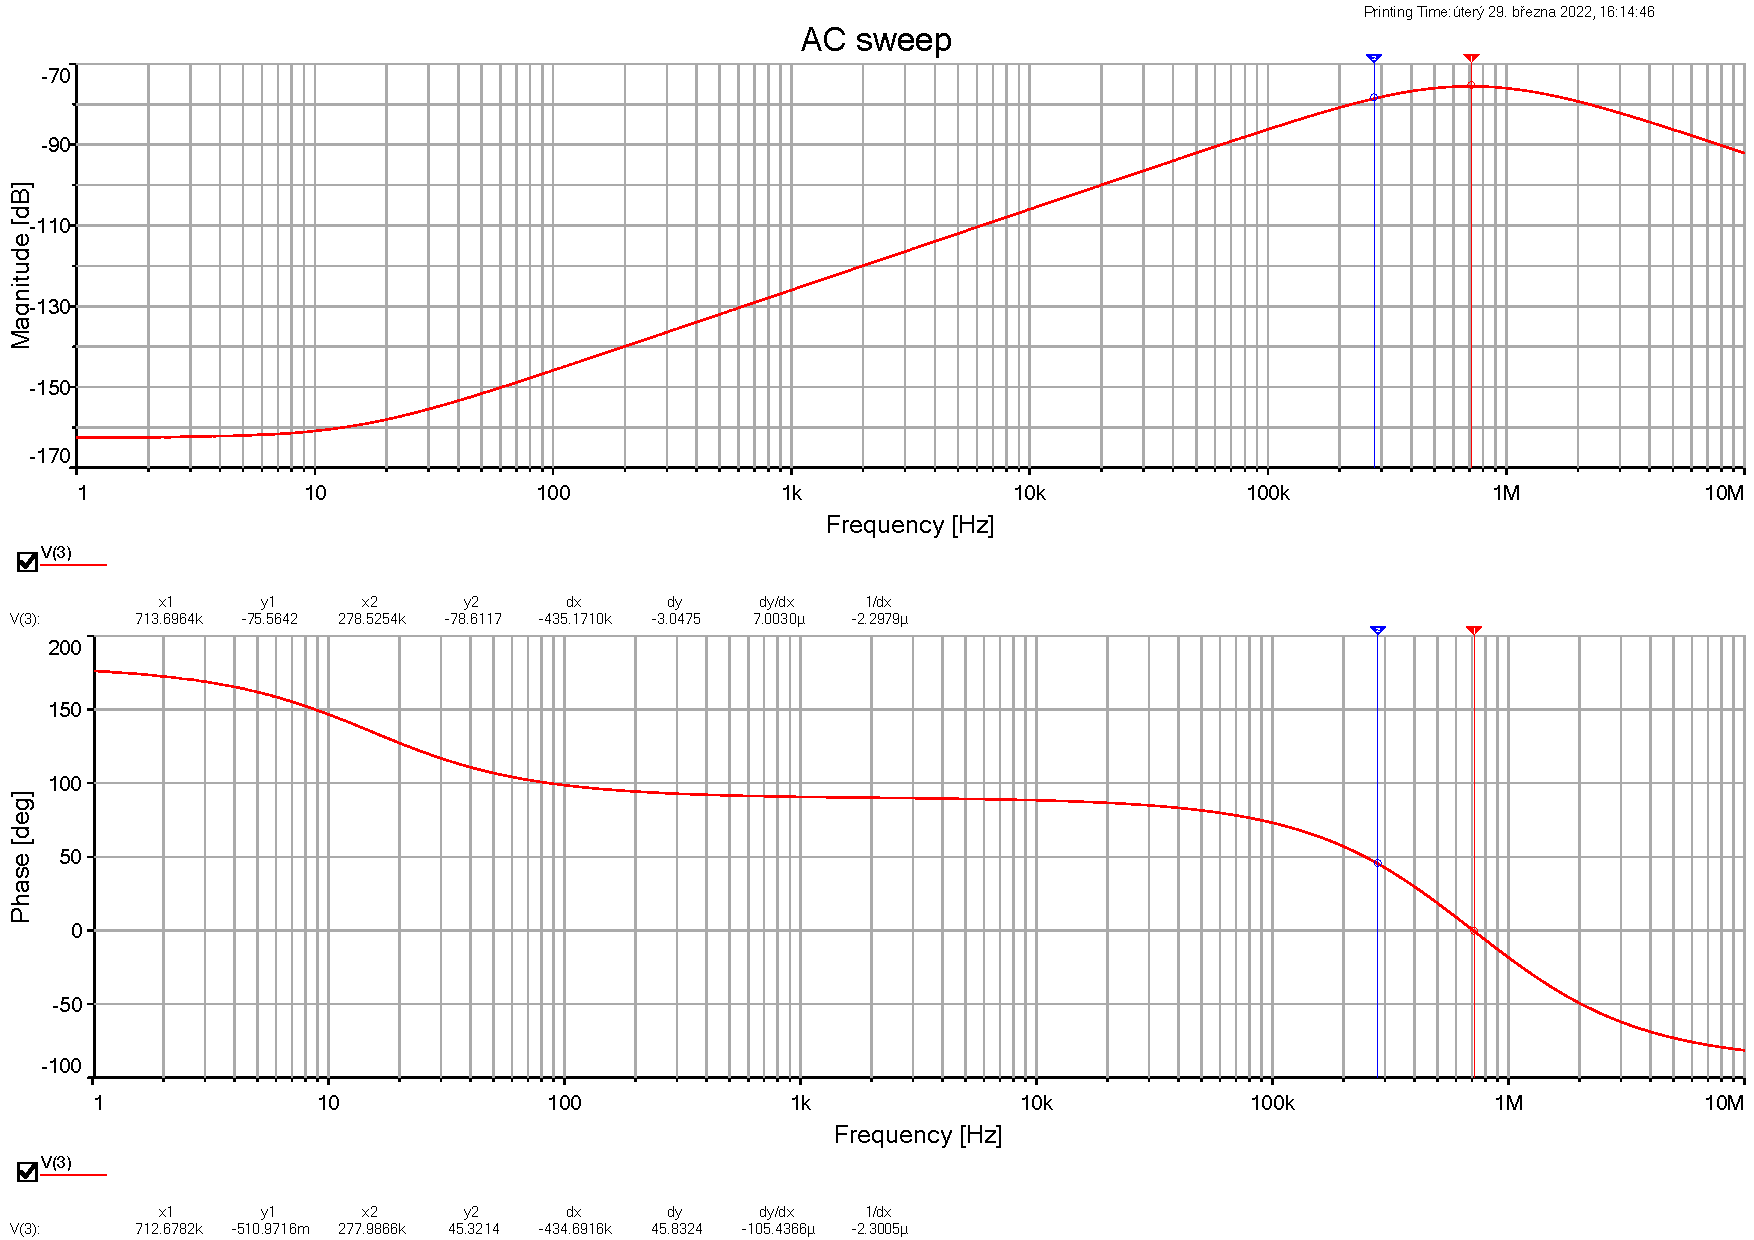
\includegraphics[width=0.92\linewidth]{bode_common_8.pdf}
    \caption{Frekvenční charakteristika souhlasného zesílení pro $G_\text{D} = 8$}
    \label{fig:bode_common_8}
\end{figure}
\newpage

\section{Doba náběhu}

\begin{figure}[h!]
    \centering
    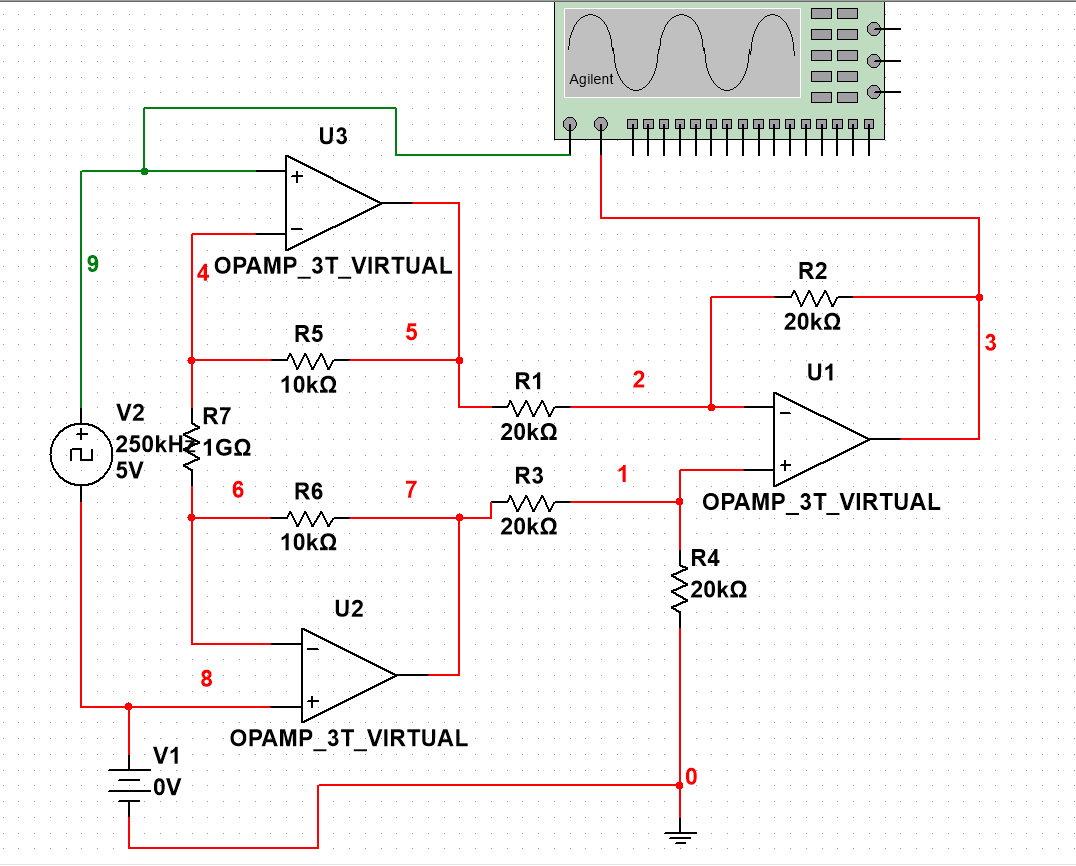
\includegraphics[width=0.7\linewidth]{rise_time_schema.png}
    \caption{Zapojení pro měření doby náběhu}
    \label{fig:rise_time_schema}
\end{figure}

S pomocí generátoru obdélníkového signálu a osciloskopu zapojeného dle schématu \ref{fig:rise_time_schema}
byly zachyceny časové průběhy vykreslené na obrázku \ref{fig:rise_time_1} pro nastavené rozdílové zesílení $G_\text{D} = 1$.
Pomocí kurzorů byla odečtena doba náběhu $T_n = 885 \si{\nano\second}$ pro $G_\text{D} = 1$. To odpovídá očekávané
době náběhu vypočtené dle vztahu $T_n \approx 0,35 / f_m$ pro $f_m \approx 417 \si{\kilo\hertz}$.

\begin{figure}[h!]
    \centering
    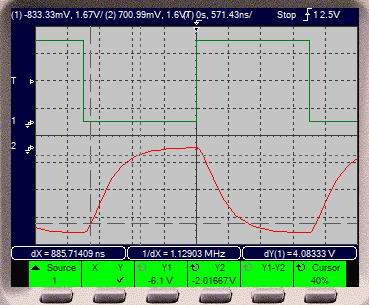
\includegraphics[width=0.6\textwidth]{rise_time_1.png}
    \caption{Doba náběhu přístrojového zesilovače pro rozdílové zesílení $G_\text{D}=1$}
    \label{fig:rise_time_1}
\end{figure}

\end{document}

